% @file dokumentace.tex
% @author Štěpán Faragula
% @brief Dokumentace semestrální práce z předmětu KIV/TI.
% @version 1.0
% @date 2023-08-01

% Document
\documentclass[12pt]{report}

% Čeština
\usepackage[utf8]{inputenc}
\usepackage[IL2]{fontenc}
\usepackage[czech]{babel}
\usepackage{fontspec}

% Formát dokumentu
\usepackage{amsmath}
\usepackage{caption}
\usepackage{textcomp}
\usepackage{xspace}
\usepackage{parskip}
\usepackage[hidelinks]{hyperref}

% Graphics
\usepackage{graphicx}
\graphicspath{{img/}}
\usepackage{fancyvrb}
\usepackage[
left=30mm, 
right=30mm, 
top=30mm, 
bottom=30mm,
]{geometry}

% Vychytávky
\usepackage{lipsum}								% Lorem impsum
\usepackage{pdflscape}							% Landscape
\usepackage{menukeys}							% Klavesy
\usepackage{algorithm}							% Algoritmus
\usepackage[noend]{algpseudocode}				% Pseudokod
\usepackage{dirtree}							% Adresarova struktura
												% Tabulky pomoci https://www.tablesgenerator.com/

% Macra
\newcommand\la{\textlangle}  					% levá závorka <
\newcommand\ra{\textrangle}						% pravá závorka >
\newcommand\laratexttt[1]{\la\texttt{#1}\ra}	% texttt v závorkách <>

\newcommand\indentt[1]{						
	\setlength\parindent{5mm}
	#1
	\setlength\parindent{0mm}
}												% odstavec

\algnewcommand{\StartComment}[1]{
	\State\(\triangleright\) #1
}												% komentar pseudokodu

\algnewcommand{\bracketbf}[1]{
	\text{(} \textbf{#1} \text{)}
}												% textbf v normalnich zavorkach ()

\newcommand\horizontalpagenumber{
	\pagestyle{empty}
	\vbox to 0pt{\vss}\vfill
	\vbox to 0pt{\baselineskip0pt
	\hbox to\linewidth{\hss}
	\baselineskip\footskip
	\hbox to\linewidth{
	\hfil\thepage\hspace{30mm}}\vss}
}

% Begin
\begin{document}
	
	% Titulní strana
	\begin{titlepage}
		\centering
		\Large
		
		
\includegraphics[width=.7\textwidth]{fav}
		
		\vspace{15mm}
		{\Huge\bfseries Semestrální práce z předmětu KIV/PT}
		
		\vspace{5mm}
		{\LARGE Sanitace nádrží}
		
		\vfill
		\raggedright
		Štěpán Faragula\\
		A21B0119P\\
		Mikuláš Mach\\
		A21B0202P
		\hfill 
		\today
	\end{titlepage}
	
	% Obsah
	\tableofcontents
	
	% Zadání
	\chapter{Zadání}
	Na \href{http://home.zcu.cz/~vais/}{http://home.zcu.cz/$\sim$vais/} v rozšiřujícím materiálu o konečných automatech prostudujte kapitoly Logické řízení a Principy softwarové implementace.
	
	Navrhněte konečněautomatový model řídícího systému níže popsaného zařízení.
	
	Sanitaci pivovarských tanků se provádí ve dvou fázích. V první fázi se přepustí roztok louhu ze zásobní nádrže do tanku. Jakmile dosáhne hladina v tanku maxima (signál LA011 nebo LA031), tzn. že dosáhne čidla LA/01 resp. LA/03, celý obsah tanku se~přečerpá pomocí čerpadla (spuštění signálem P1, vypnutí signálem P0) zpět do zásobní nádrže. Ve druhé fázi se tank naplní vodou a poté se otevře výpustný ventil (otevření ventilu i signálem Vi1, uzavření signálem Vi0) a tank je proplachován vodou tak dlouho, dokud pH na výtoku neklesne pod zadanou mez (signál Q0). Celý cyklus sanitace je ukončen když hladina v nádrži klesne pod dolní mez (LA020 nebo LA040), tzn. že klesne pod čidlo LA/02 resp. LA/04. Operátor spouští sanitaci tanku A nebo B stisknutím tlačítka A (signál A) nebo B (signál B). Jestliže tank není prázdný, nelze nezačínat sanitaci, ale výstupním signálem Z1 rozsvítit signální žárovku. Žárovka má svítit do té doby, dokud není příslušný tank vyprázdněn ručním ovládáním.
	
	Model řídícího automatu realizujte softwarově na základě principů popsaných v materiálu. Všechny signály od čidel modelujte vstupy od klávesnice, řídící signály a informaci o stavu vypisujte textově na obrazovku.
	
	Automat popište přechodovým grafem. Pro zakreslení přechodového grafu použijte software JFLAP (\href{https://www.jflap.org/}{https://www.jflap.org/}).
	
	Technologické schéma je vidět na obrázku \ref{fig:schema} na straně \pageref{fig:schema}.
	
	\begin{figure}
		\centering
		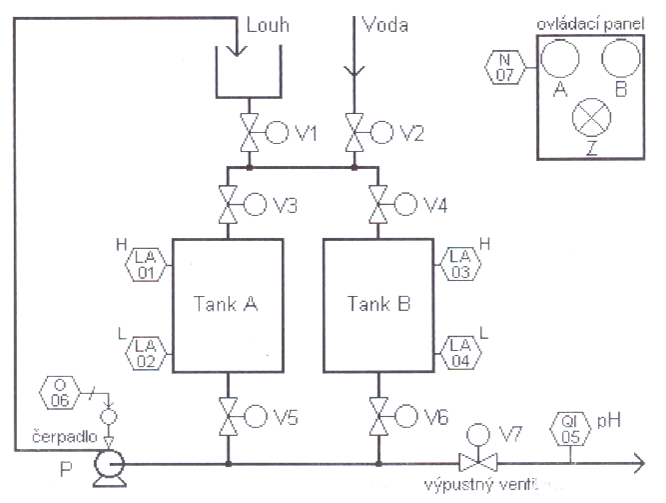
\includegraphics[width=0.6\textheight]{schema}
		\caption{Technologické schéma}
		\label{fig:schema}
	\end{figure}
	
	% Analýza úlohy
	\chapter{Analýza úlohy}
	
	% Automatový model
	\chapter{Automatový model}
	
	\section{Vstupní signály}
	Očekává se, že systém bude řízen pouze dvěma tlačítky, které začnou čištění jednotlivých nádrží. Dále očekáváme, že pokud nejsou nádrže vyprázdněny před sanitací, tak je operátor vypustí ručním ovládáním. Automat tedy bude mít 3 vstupní aktivní signály: 
	
	\begin{itemize}
		\item \texttt{N\_A} – spustí čištění nádrže A
		\item \texttt{N\_B} – spustí čištění nádrže B
		\item \texttt{RUC} – vypustí obsah nádrží 
	\end{itemize}

	Obě nádrže mají čidla, které snímají horní a dolní mez hladiny. Dále je na výtoku umístěn snímač pH. Každé čidlo může nabývat dvou stavů – není aktivní (\texttt{0}), aktivní (\texttt{1}). Čidla nádrže jsou v aktivním stavu, pokud platí \texttt{hladina kapaliny v nádrži >= snímaná mez}. Snímač výtoku je v aktivním stavu, pokud platí \texttt{pH na výtoku >= snímaná mez}. Automat tedy bude mít 5 pasivních vstupních signálů, které mohou nabývat dvou různých hodnot:

	\begin{itemize}
		\item \texttt{LA1\_i} – horní snímač hladiny nádrže A
		\item \texttt{LA2\_i} – dolní snímač hladiny nádrže A
		\item \texttt{LA3\_i} – horní snímač hladiny nádrže B
		\item \texttt{LA4\_i} – dolní snímač hladiny nádrže B
		\item \texttt{Q\_i} – snímač hodnoty pH na výtoku
	\end{itemize}

	Všechny vstupní signály jsou vidět v tabulce \ref{tab:vstupni} na straně \pageref{tab:vstupni}.

	\begin{table}[]
		\centering
		\begin{tabular}{lll}
			\hline
			\multicolumn{1}{c}{Vstupní signál} 	& \multicolumn{1}{c}{Druh} & \multicolumn{1}{c}{Popis}    \\ \hline
			RUC                                 & Aktivní                  & Ruční vypouštění nádrží      \\
			N\_A                                & Aktivní                  & Spuštění sanitace nádrže A   \\
			N\_B                                & Aktivní                  & Spuštění sanitace nádrže B   \\ \hline
			LA1\_i                              & Pasivní                  & Horní čidlo hladiny nádrže A \\
			LA2\_i                              & Pasivní                  & Dolní čidlo hladiny nádrže A \\
			LA3\_i                              & Pasivní                  & Horní čidlo hladiny nádrže B \\
			LA4\_i                              & Pasivní                  & Dolní čidlo hladiny nádrže B \\
			Q\_i                                & Pasivní                  & Kontrola pH na výtoku        \\ \hline
		\end{tabular}
		\caption{Vstupní signály}
		\label{tab:vstupni}
	\end{table}

	\section{Výstupní signály}
	Jedná se o signály, které vykonají akci při přechodu mezi stavy. V modelu budeme ovládat celkem 7 ventilů, kde každý může být ve stavu zavřen (\texttt{0}) nebo otevřen (\texttt{1}). Stejným způsobem budeme ovládat také žárovku a čerpadlo. Všechny výstupní signály jsou vidět v tabulce \ref{tab:ridici}.
	
	\begin{table}[]
		\centering
		\begin{tabular}{ll}
			\hline
			\multicolumn{1}{c}{Řídící signál} 	& \multicolumn{1}{c}{Popis}  	\\ \hline
			V1\_i          					  	& Ventil 1      			   	\\
			V2\_i         					  	& Ventil 2      				\\
			V3\_i          					  	& Ventil 3      				\\
			V4\_i          					  	& Ventil 4      				\\
			V5\_i          					  	& Ventil 5      				\\
			V6\_i          					  	& Ventil 6      				\\
			V7\_i          					  	& Ventil 7      				\\
			P\_i          					  	& Čerpadlo      				\\
			Z\_i          					  	& Žárovka      					\\ \hline
		\end{tabular}
		\caption{Řídící signály}
		\label{tab:ridici}
	\end{table}	

	\section{Stavy modelu}
	Náš navržený model bude obsahovat celkem 15 stavů, jsou popsány v tabulce \ref{tab:stavy} na straně \pageref{tab:stavy}.
			
	\begin{table}[]
		\centering
		\begin{tabular}{ll}
			\hline
			\multicolumn{1}{c}{Stav} 	 & \multicolumn{1}{c}{Popis}      \\ \hline
			0                            & Počáteční stav				  \\
			1                            & Nádrže nejsou prázdné          \\
			2                            & Ruční vypouštění nádrže A   	  \\ 
			3                            & Ruční vypouštění nádrže B   	  \\ 
			4                            & Systém čeká na vstup 		  \\ \hline
			5A                           & Napouštění louhem nádrže A     \\
			6A                           & Vypouštění louhu nádrže A      \\
			7A                           & Napouštění vodou nádrže A      \\
			8A                           & Proplachování vodou nádrže A   \\
			9A                           & Vypouštění vody nádrže A       \\ \hline
			5B                           & Napouštění louhem nádrže B     \\
			6B                           & Vypouštění louhu nádrže B      \\
			7B                           & Napouštění vodou nádrže B      \\
			8B                           & Proplachování vodou nádrže B   \\
			9B                           & Vypouštění vody nádrže B       \\ \hline
		\end{tabular}
		\caption{Stavy modelu}
		\label{tab:stavy}
	\end{table}
		
	\section{Přechodový graf}
	Pro řídící systém jsme navrhli přechodový graf, který je znázorněn na obrázku \ref{fig:graf} na straně \ref{fig:graf}.
		
	\newgeometry{margin=5mm}  
	\begin{landscape}
		\begin{figure}
			\centering
			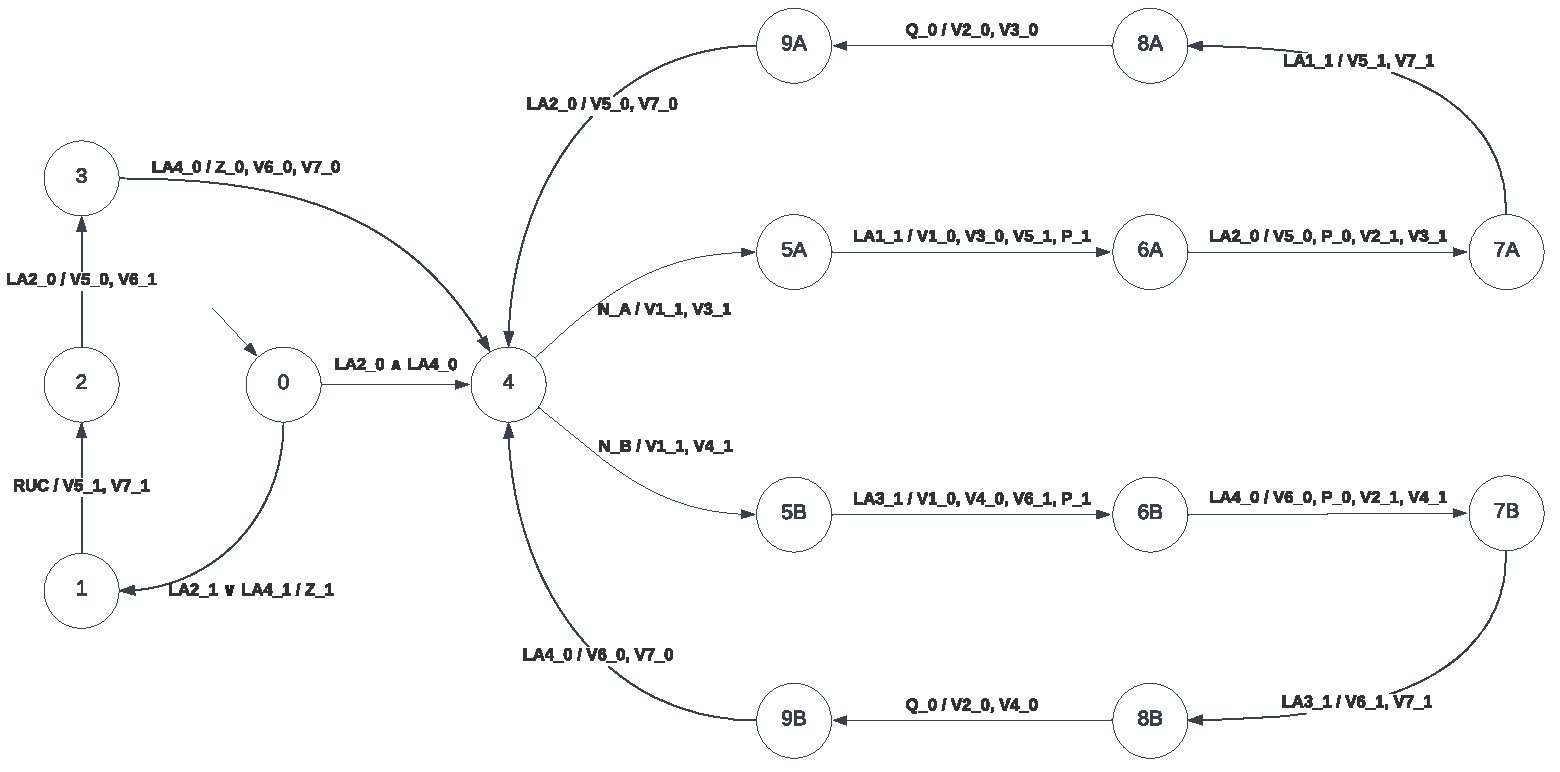
\includegraphics[width=1.3\textwidth]{graf}
			\caption{Graf přechodu}
			\label{fig:graf}
			\horizontalpagenumber
			\end{figure}
	\end{landscape}
	\restoregeometry
	
	% Implementace
	\chapter{Implementace}
	Konečný automat je implementován v programovacím jazyce Java verze 17.
	
	\section{Zdrojové soubory}
	Aplikace se skládá celkem z 5 souborů obsahující kód. Jejich funkce je následující:
	
	 \begin{itemize}
		\item \texttt{Main} – hlavní třída, bere vstup od uživatele a předává ho automatu
		\item \texttt{Stroj} – třída reprezentující řídící systém (konečný automat)
		\item \texttt{StrojStav} – výčtový typ reprezentující stavy konečného automatu
		\item \texttt{StrojVstup} – výčtový typ reprezentující signály konečného automatu
		\item \texttt{StrojVystup} – výčtový typ reprezentující řídící signály konečného automatu
	\end{itemize}	
	
	\section{Automat}
	V této třídě jsme při implementaci postupovali doporučenou metodou. Automat si uchovává svůj stav, stavové proměnné a zadaný vstup. Dále obsahuje přechodovou a výstupní tabulku, podle kterými se automat řídí.
	
	Při spuštění programu naplníme tabulky metodou \texttt{inic\_tab()} a nastavíme stav a stavové proměnné automatu pomocí \texttt{inic\_stav()}. Následuje nekonečná smyčka, kde automatu předáváme vstup od uživatele pomocí metody \texttt{vstup\_znaku()}. O tom, jestli se něco vykoná po zadání vstupu, rozhodují metody \texttt{vyst\_akce()} a \texttt{transf\_akce()}. Ty se podívají do tabulky, podle které provedou akci.
	
	% Uživatelská příručka
	\chapter{Uživatelská příručka}
	Program je zamýšlen pro běh v konzoli, nejedná se tedy o aplikaci s grafickým rozhraním.
	
	\section{Spuštění programu}
	Před spuštěním se očekává, že má uživatel na svém počítači nainstalovaný jazyk Java. Program nepotřebuje žádné knihovny ani speciální přepínače pro běh. Spouštění je jednoduché, stačí poklepat na soubor \texttt{TI\_Semestralka.jar}. 
	
	V případě spouštění programu z konzole zadáme následující příkaz:
	
	\indentt{
		\texttt{java -jar TI\_Semestralka.jar} \keys{\return}
	}
	
	Po spuštění se vypíše do konzole nápověda pro ovládání a automat se uvede do počátečního stavu. Názorná ukázka je vidět na obrázku \ref{fig:start} na straně \pageref{fig:start}. 
	
	\section{Ovládání programu}
	Ovládání je velmi intuitivní, u každého stavu se vypíše nabídka relevantních vstupů, poté se čeká na uživatele, který si zvolí. Pokud by daný vstup změnil stav automatu, vypíšou se všechny výstupní akce transformace. Program přijímá pouze číselný vstup. V kterýkoliv okamžik můžeme vypsat hodnoty stavových proměnných číslem \texttt{0}. Jakékoliv záporné číslo (ne jenom \texttt{-1}) ukončí program. Ukázkový běh programu je vidět na obrázku \ref{fig:beh} na straně \pageref{fig:beh}.

	\begin{figure}
		\centering
		\BVerbatimInput{img/spusteni.txt}
		\caption{Zapnutí programu}
		\label{fig:start}
	\end{figure}

	\begin{figure}
		\centering
		\BVerbatimInput{img/beh.txt}
		\caption{Ukázkový běh programu}
		\label{fig:beh}
	\end{figure}


	% Závěr
	\chapter{Závěr}
	
\end{document}
